\documentclass{beamer}
\mode<presentation>
%\mode<handout>% para impressão
{
\usetheme{Warsaw}                          %Há vários outros temas disponíveis
\setbeamercovered{transparent}
}
\usepackage{listings}

\lstset{language=c++,
                basicstyle=\ttfamily,
                keywordstyle=\color{blue}\ttfamily,
                stringstyle=\color{red}\ttfamily,
                commentstyle=\color{green}\ttfamily,
								showspaces=false,
								showstringspaces=false,
								tabsize=1,
                morecomment=[l][\color{magenta}]{\#}
}

\usepackage{graphicx}
\usepackage[absolute,overlay]{textpos}

\title[SQLite]{SQLite}
\author{Felipe L. Pinheiro}
\institute{Universidade de Brasília\\
						Instituto de Ciências Exatas\\
            Departamento de Ciência da Computação\\
						Metodologia de pesquisa}

\begin{document}

\begin{frame}
	\titlepage
\end{frame}

\begin{frame}
\begin{figure}
    \centering
    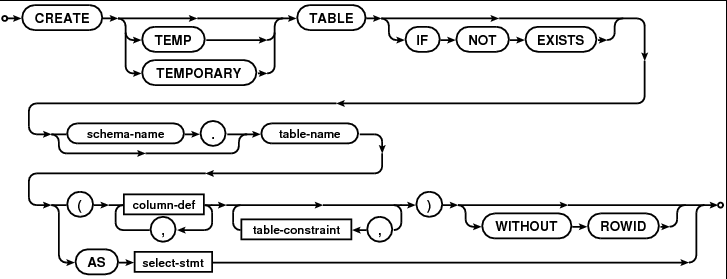
\includegraphics[width=0.8\linewidth]{create-table-stmt}
    \caption{Esquema do statment CREATE TABLE}
    \label{fig:create-table}
\end{figure}
\end{frame}

\begin{frame}
\begin{figure}
    \centering
    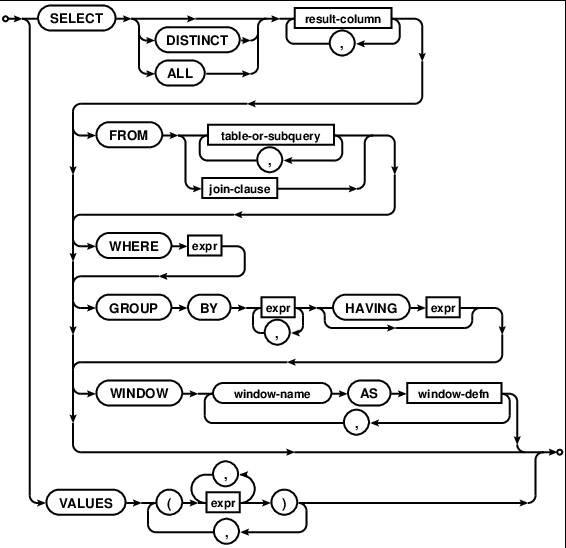
\includegraphics[width=0.6\linewidth]{select-core}
    \caption{Esquema do comando SELECT}
    \label{fig:select}
\end{figure}	
\end{frame}


\begin{frame}[fragile]{Exemplo}
\begin{lstlisting}
static async Task Main(){
	var connection = new SqliteConnection
		("Data Source=StreamingSample.db");
	connection.Open();

	var createCommand = connection.CreateCommand();
	createCommand.CommandText =
	@"CREATE TABLE data (
		id INTEGER PRIMARY KEY AUTOINCREMENT,
		value BLOB
	)";
	createCommand.ExecuteNonQuery();

\end{lstlisting}
\end{frame}

\begin{frame}[fragile]{Exemplo}
\begin{lstlisting}
	using (var inputStream = File.OpenRead
	("input.txt")){
		var insertCommand = connection.CreateCommand();
		insertCommand.CommandText =
		@"INSERT INTO data(value) 
			VALUES (zeroblob($length));
			SELECT last_insert_rowid();";
			insertCommand.Parameters.AddWithValue
		("$length", inputStream.Length);
		var rowid = (long)insertCommand
			.ExecuteScalar();

\end{lstlisting}
\end{frame}

\begin{frame}[fragile]{Exemplo}
\begin{lstlisting}

		using (var writeStream = new SqliteBlob
		(connection, "data", "value", rowid)){
			Console
				.WriteLine("Writing the large object...");
			
			await inputStream.CopyToAsync(writeStream);
		}
	}

\end{lstlisting}
\end{frame}

\begin{frame}[fragile]{Exemplo}
\begin{lstlisting}

	using (var outputStream = Console
		.OpenStandardOutput()){
		var selectCommand = connection
			.CreateCommand();
		selectCommand.CommandText =
		@"
		SELECT id, value
		FROM data
		LIMIT 1
		";
		
\end{lstlisting}
\end{frame}

\begin{frame}[fragile]{Exemplo}
\begin{lstlisting}
		
		using (var reader = selectCommand.ExecuteReader()){
			while (reader.Read()){
				using (var readStream = reader.GetStream(1)){
					Console.WriteLine("Reading the large object...");
					await readStream.CopyToAsync(outputStream);
				}
			}
		}
	}
	
\end{lstlisting}
\end{frame}

\begin{frame}[fragile]{Exemplo}
\begin{lstlisting}

	connection.Close();
	File.Delete("StreamingSample.db");
}
	
\end{lstlisting}
\end{frame}

\end{document}